\newpage
\section[Numerical Sequences and Series]{\hyperlink{toc}{Numerical Sequences and Series}}
\subsection{Sequences}
We begin by formally defining a sequence.
\begin{ndef}{: Sequences}{}
    Let $X$ be a metric space. A \textbf{sequence} is a function $f: \NN \mapsto X$. We can denote a term in the sequence as $f(n) = x_n$, or the entire sequence as $\set{x_n}_{n=1}^\infty$, $\set{x_n}$, $(x_n)$, or $\set{x_1, x_2, x_3 \ldots}$. 
\end{ndef}
\noindent We now discuss the notion of convergence of a sequence. Intuitively, we can equate convergence with the notion of points getting closer together.
\begin{definition}{Convergence of Sequences}{3.1}
    A sequence $\set{p_n}_{n=1}^\infty$ \textbf{converges} to $p \in X$ if for all $\e > 0$, there exists $N \in \NN$ such that $n \geq N$ implies $d(p_n, p) < \e$. In this case, we say that $\set{p_n}$ converges to $p$, or that $p$ is the limit of $\set{p_n}$, and denote this as $p_n \rightarrow p$ or $\lim_{n \rightarrow \infty} p_n = p$. If $\set{p_n}$ does not converge, we say it \textbf{diverges}.
\end{definition}
\noindent To phrase this definition in another way, we fix some $\e > 0$, and then we have that all points in the sequence past some $N \in \NN$ are contained in the neighbourhood $N_\e(p)$. In practice, it can be difficult to apply this definition of convergence if we don't know what the limiting $p$ is, as the definition implicitly uses the value of the limit. We will later discuss another definition of convergence (in $\RR^k$) that does not use the value of the limit.
\begin{figure}[htbp]
    \centering
    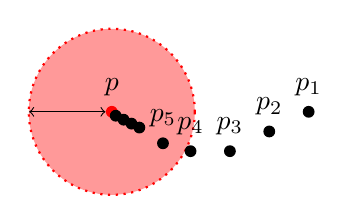
\begin{tikzpicture}[mycirc/.style={circle,fill, minimum size=0.15cm, inner sep = 0pt}]
        \draw[red, dotted, thick, fill = white!60!red] (-1, 0) circle (30pt);
        \node[mycirc, label=above:{$p$}, fill = red] at (-1, 0) {};
        \node[mycirc, label=above:{$p_1$}] at (1.5, 0) {};
        \node[mycirc, label=above:{$p_2$}] at (1, -0.25) {};
        \node[mycirc, label=above:{$p_3$}] at (0.5, -0.5) {};
        \node[mycirc, label=above:{$p_4$}] at (0, -0.5) {};
        \node[mycirc, label=above:{$p_5$}] at (-0.35, -0.4) {};
        \node[mycirc] at (-0.65, -0.2) {};
        \node[mycirc] at (-0.75, -0.15) {};
        \node[mycirc] at (-0.85, -0.1) {};
        \node[mycirc] at (-0.95, -0.05) {};
        \draw[<->] (-1.08, 0) -- (-2.05, 0);
        \node[label=above:{$\e$}] at (-1.5, -0.15) {};
    \end{tikzpicture}
    \caption{Visualization of a sequence $\set{p_n} \subset \RR^2$ converging to a point $p$. For the $\e > 0$ shown in the picture, we have that all points of the sequence past $N = 5$ lie in the open disk of radius $\e$ around $p$.}
    \label{fig15}
\end{figure}

\noindent As a remark, consider that convergence can depend on our choice of metric space; for example, $\set{\frac{1}{n}}$ as a sequence in $\RR$ converges to $0$, but the same sequence in the strictly positive reals ($\RR^+ = \set{x \in \RR: x > 0}$) does not converge.

Another interesting example (that again shows us the importance of the choice of metric space). Is $\RR$ equipped with the discrete metric. A question we can ask is ``given some points $p \in \RR$, what sequences converge to $p$?'' The answer turns out to be eventually constant sequences only; that is, sequences for which $p_n = p$ for $n \geq N$ for some $N$. 
\begin{proof}
    If $p_n \rightarrow p$, then setting $\e = \frac{1}{2}$, we have that there exists $N \in NN$ such that for all $n \geq N$, $d(p_n, p) < \e = \frac{1}{2}$. Under the discrete metric, this is only possible if $p_n = p$. 
\end{proof}
This of course is a strikingly different picture for $\RR$ with the standard metric of $d(x, y) = \abs{x - y}$. For example, the sequnce $p_n = \frac{1}{n}$ has no term equal to zero, but converges to $p = 0$. The takeaway message here can be that in the Euclidean metric, points can ``get closer'' but in the discrete metric, they cannot.

\stepcounter{rudin}
\begin{theorem}{}{3.3}
    Suppose $\set{s_n}, \set{t_n}$ are complex sequences that converge, with $\linf s_n \rightarrow s$ and $\linf t_n \rightarrow t$. Then:
    \begin{enumerate}
        \item $\linf(s_n + t_n) = s + t$.
        \item $\linf cs_n = cs$ and $\linf (c + s_n) = c + s$ for all $c \in \CC$.
        \item $\linf s_nt_n = st$
        \item $\linf \frac{1}{s_n} = \frac{1}{s}$ provided $s \neq 0$ and $s_n \neq 0$ for all $n$.
    \end{enumerate}
\end{theorem}
\begin{nproof}
    \begin{enumerate}
        \item Let $\e > 0$. There exist $N_1, N_2 \in \NN$ such that $\abs{s_{n_1} - s} < \frac{\e}{2}$ for $n_1 \geq N_1$ and $\abs{t_{n_2} - t} < \frac{\e}{2}$ for $n_2 \geq N_2$. Take $N = \max{N_1, N_2}$, and using the triangle inequality, it follows that for $n \geq N$:
        \begin{align*}
            \abs{(s_n + t_n) - (s + t)} \leq \abs{s_n - s} + \abs{t_n - t} < \frac{\e}{2} + \frac{\e}{2} = \e
        \end{align*} 
        We conclude that $\linf (s_n + t_n) = s + t$. 
        \item Let $\e > 0$. If $c = 0$ then the first sequence trivially converges to $0$, so suppose that $c \neq 0$. There exists $N$ such that $\abs{s_n - s} < \frac{\e}{\abs{c}}$ for $n \geq N$, so it follows that:
        \begin{align*}
            \abs{cs_n - cs} = \abs{c}\abs{s_n - s} < \abs{c}\frac{\e}{\abs{c}} = \e.
        \end{align*} For the second identity, we have that $c_n \rightarrow c$ for any constant sequence $c_n = c$ so we may apply (a).
        \item Let $\e > 0$. There exist $N_1, N_2$ such that $\abs{s_{n_1} - s} < \sqrt{2}$ for $n_1 \geq N_1$ and $\abs{t_{n_2} - t} < \sqrt{2}$ for $n_2 \geq N_2$. We then consider that:
        \begin{align*}
        s_nt_n - st = (s_n - s)(t_n - t) + s(t_n - t) + t(s_n - s)
        \end{align*}
        For $n \geq N = \max{N_1, N_2}$, we have that:
        \begin{align*}
            (s_n - s)(t_n - t) < \e
        \end{align*}
        And we hence observe that $\linf (s_n - s)(t_n - t) = 0$. We can then use (a) and (b) to find that:
        \begin{align*}
            \linf s(t_n - t) = 0, \quad \linf t(s_n - s) = 0
        \end{align*}
        So we conclude that $\linf (s_nt_n - st) = 0$ and hence $s_nt_n \rightarrow st$.
    \end{enumerate}
\end{nproof}
\begin{nproofcont}
    \begin{enumerate}
        \setcounter{enumi}{3}
        \item Choose $m$ such that $\abs{s_n - s} < \frac{1}{2}\abs{s}$ if $n \geq m$. We then have that $\abs{s_n} > \frac{1}{2}\abs{s}$ for $n \geq m$. Let $\e > )0$. Then, there exists $N$ with $N > m$ such that for $n \geq N$:
        \begin{align*}
            \abs{s_n - s} < \frac{1}{2}\abs{s}^2\e
        \end{align*}
        Hence, for $n \geq N$:
        \begin{align*}
            \abs{\frac{1}{s_n} - \frac{1}{s}} = \abs{\frac{s_n - s}{s_ns}} < \frac{2}{\abs{s}^2}\abs{s_n - s} < \e
        \end{align*}
        \qed
    \end{enumerate}
\end{nproofcont}

\begin{nlemma}{: Squeeze Lemma}{}
    Let $\set{x_n}$, $\set{s_n}$ be real-valued sequences. Then, if $0 \leq x_n \leq s_n$ for all $n$, and $\linf s_n = 0$, then $\linf x_n = 0$.
\end{nlemma}
\begin{nproof}
    Let $\e > 0$. Choose $N \in \NN$ such that $n \geq N$ implies $0 \leq s_n < \e$. Then, we have that for $n \geq N$, $0 \leq x_n \leq s_n < \e$ and hence $x_n \rightarrow 0$ as claimed. \qed
\end{nproof}

\noindent Note that we can prove a more generalized version of the Squeeze Lemma. Suppose we have sequences $\set{l_n}, \set{x_n}, \set{u_n}$ such that $l_n \leq x_n \leq u_n$ for all $n$ and $\linf l_n = \linf u_n = L \in \RR$. Then, $\linf x_n = L$.
\begin{proof}
    We have that $0 \leq a_n - l_n \leq u_n - l_n$. We have that $\linf u_n - l_n = 0$ by Theorem \ref{thm:3.3}(a), so by the (original) Squeeze Lemma we have that $\linf a_n - l_n = 0$. It then follows that $\linf a_n = \linf l_n = L$ as claimed.
\end{proof}

\setcounter{rudin}{19}
\begin{theorem}{}{3.20}
    \begin{enumerate}
        \item Let $p > 0$. Then, $\linf \frac{1}{n^p} = 0$.
        \item Let $p > 0$. Then, $\linf \sqrt[n]{p} = 1$.
        \item $\linf \sqrt[n]{n} = 1$.
        \item Let $p > 0$ and $\alpha \in \RR$. Then, $\linf \frac{n^\alpha}{(1+p)^n} = 0$.
        \item Let $\abs{x} < 1$. Then, $\linf x^n = 0$. 
    \end{enumerate}
\end{theorem}
\begin{nproof}
    \begin{enumerate}
        \item Let $\e > 0$. Choose $N$ such that $\frac{1}{N^p} < \e$, namely $N > \left(\frac{1}{\e}\right)^{1/p}$. Then, for $n \geq N$, $\frac{1}{n^p} < \frac{1}{N^p} < \e$. 
        
        \item If $p = 1$, the sequence is constant and the conclusion immediate. 
        
        If $p > 1$, then let $x_n = \sqrt[n]{p} - 1$. We then have that:
        \begin{align*}
            p = (x_n + 1)^n = \sum_{k=0}^n \binom{n}{k}x_n^k \geq nx_n
        \end{align*}
        Where the second equality follows from the binomial theorem (where $\binom{n}{k} = \frac{n!}{k!(n-k)!}$), and the inequality follows by considering that we just keep the $k = 1$ term (and the series is non-negative). Hence, we have that $x_n \leq \frac{p}{n}$, and $x_n \rightarrow 0$ by (a). 
        
        If $p < 1$, then let $q = \frac{1}{p} > 1$. Then, $\sqrt[n]{q} \rightarrow 1$ by the argument above. By Theorem \ref{thm:3.3}(d), we then have that $\sqrt[n]{p} = \frac{1}{\sqrt[n]{q}} \rightarrow \frac{1}{1} = 1$.

        \item Let $x_n = \sqrt[n]{n} - 1$. Then, we have that:
        \begin{align*}
            n = (x_n + 1)^n = \sum_{k=0}^n\binom{n}{k}x_n^k \geq \frac{n(n-1)}{2}x_n^2
        \end{align*}
        Where the inequality follows from keeping the $k = 2$ term only. We then have that $x_n \leq \sqrt{\frac{2}{n-1}}$ and hence $x_n \rightarrow 0$ by the Squeeze Lemma.
        \item We want to show $\frac{n^\alpha}{(1+p)^n} \rightarrow 0$; we therefore want an upper bound on the expression, and hence a lower bound on $(1+p)^n$. Applying the Binomial Theorem we have that:
        \begin{align*}
            (1+p)^n = \sum_{k=0}^n\binom{n}{k}p^k = \left((n)(n-1)(n-2)\cdots(n-k+1)\right)\frac{p^k}{n!}
        \end{align*}
        Now, we pick $k > \alpha$. For $2n > k$, we then have that:
        \begin{align*}
            (1+p)^n \geq \left(\frac{n}{2}\right)^k\frac{p^k}{k!}
        \end{align*}
        We therefore have that:
        \begin{align*}
            \frac{n^\alpha}{(1+p)^k} \leq \frac{2^kk!}{p^k}n^{\alpha - k} \rightarrow 0
        \end{align*}
        And the claim follows by the Squeeze Lemma.
        
        \item Taking $\alpha = 0$ in (d), the claim follows by setting $\abs{x} = \frac{1}{1+p} < 1$ (as $p > 0$) and recognizing that $x_n \rightarrow 0 \iff \abs{x^n} = \abs{x}^n \rightarrow 0$. \qed
    \end{enumerate}
\end{nproof}

\subsection{Subsequences}

\setcounter{rudin}{1}
\begin{theorem}{}{3.2}
    Let $\set{p_n}$ be a sequence in $X$.
    \begin{enumerate}
        \item $p_n \rightarrow p$ in $X$ if and only if for all $r > 0$, $N_r(p)$ contains all but finitely many points of $\set{p_n}$.
        \item If $p_n \rightarrow p$ and $p_n \rightarrow p'$ then $p = p'$. In other words, the limit is unique.
        \item If $\set{p_n}$ is convergent, then it is bounded (that is, for any $q \in X$ there exists $M \in \RR$ such that $d(q, p_n) \leq M$ for all $n \in \NN$).
        \item If $E \subset X$ has a limit point $p$, then there exists $\set{p_n}$ in $E$ such that $p_n \rightarrow p$. 
    \end{enumerate}
\end{theorem}
\begin{nproof}
    \begin{enumerate}
        \item The claim follows immediately from the definition of convergence; for any $r = \e > 0$, there exists $N \in \NN$ such that $N_r(p)$ contains $\set{p_n: n \geq N}$.
        \item There exist $N_1, N_2$ such that $d(p, p_{n_1}) < \frac{\e}{2}$ if $n_1 \geq N_1$ and $d(p, p_{n_2}) < \frac{\e}{2}$ if $n_2 \geq N_2$. Then for $n \geq N = \max{N_1, N_2}$ we have (using the triangle inequality) that:
        \begin{align*}
            d(p, p') \leq d(p, p_n) + d(p_n, p') < \frac{\e}{2} + \frac{\e}{2} = \e
        \end{align*}
        Since $\e$ is arbitrary, $d(p, p') = 0$ and hence $p = p'$.

        \item If $p_n \rightarrow p$, there exists $N$ such that $d(p_n, p) < 1$ for all $n \geq N$. Set:
        \begin{align*}
            r = \max\set{1, d(p_1, p), d(p_2, p), \ldots ,d(p_{N-1}, p)}
        \end{align*}
        For any $q \in X$, we then have that:
        \begin{align*}
            d(q, p_n) \leq d(q, p) + d(p, p_n) \leq d(q, p) + r
        \end{align*}
        so the claim follows with $M = r + d(q, p) + 1$.
        \item Pick $p_n \in E$ such that $d(p_n, p) < \frac{1}{n}$. Let $\e > 0$, and $N > \frac{1}{\e}$. Then, $n \geq N$ implies $\frac{1}{n} \leq \frac{1}{N} < \e$ and hence $d(p_n, p) < \e$ for all $n \geq N$, and hence $p_n \rightarrow p$ as desired. \qed
    \end{enumerate}
\end{nproof}

\setcounter{rudin}{4}
\begin{definition}{Subsequences}{3.5}
    Given $\set{p_n}$ and $n_1 < n_2 < n_3 < \ldots$, we say that $\set{p_{n_j}}$ is a \textbf{subsequence} of $\set{p_n}$.
\end{definition}

\noindent We first consider some examples. Let $p_n = n$. Then some valid subsequences of $\set{p_n}$ are $\set{1, 2, 3, 4, 5, \ldots}$ (the original sequence), $\set{1, 3, 5, 7, \ldots}$ (the odds), $\set{2, 3, 5, 7, 11, 13, \ldots}$ (the primes). Next, let $p_n = i^n$. We have that $\set{p_n} = \set{i, -1, -i, 1, i, -1, -i, 1, \ldots}$ which is clearly divergent. However, the subsequences $\set{i, i, i, \ldots}$, $\set{-1, -1, -1, \ldots}$, $\set{-i, -i, -i, \ldots}$ and $\set{1, 1, 1, \ldots}$ are all convergent! It is hence possible for a divergent sequence to have a convergent subsequence.

\begin{nlemma}{}{}
    If $p_n \rightarrow p$, then every subsequence of $\set{p_n}$ converges to $p$. 
\end{nlemma}

\begin{nproof}
    Suppose $p_n \rightarrow p$ and let $\set{p_{n_j}}$ be a subsequence of $p_n$. Let $\e > 0$. Then, there exists some $N \in \NN$ such that $d(p, p_n) < \e$ if $n \geq N$. Hence, $d(p, p_{n_j}) < \e$ if $n_j \geq N$ and hence $p_{n_j} \rightarrow p$. \qed
\end{nproof}

\begin{theorem}{}{3.6}
    \begin{enumerate}
        \item If $\set{p_n} \subset X$ with $X$ compact, then $\set{p_n}$ has a convergenct subsequence.
        \item If $\set{p_n} \subset \RR^k$ and $\set{p_n}$ is bounded, then $\set{p_n}$ has a convergent subsequence.
    \end{enumerate}
\end{theorem}
\begin{nproof}
    \begin{enumerate}
        \item Let $E$ be the range of $\set{p_n}$. If $E$ is finite, then there exists $x \in X$ and $n_1 < n_2 < n_3 < \ldots$ such that $p_{n_j} = x$ for all $j$. Therefore $p_{n_j} \rightarrow x$ and we are done. If $E$ is infinite, then by compactness, $E \subset X$ has a limit point in $X$ by Theorem \ref{thm:2.37}. By Theorem \ref{thm:3.2}(d) there exists a sequence $\set{p_{n_j}}$ in $E$ such that $p_{n_j} \rightarrow p$.
        \item By Theorem \ref{thm:2.41}, $E$ (being bounded) lies in a compact subset of $\RR^k$. We then apply (a). \qed
    \end{enumerate}
\end{nproof}

\subsection{Cauchy Sequences and Completeness}

\setcounter{rudin}{7}
\begin{definition}{Cauchy Sequences}{3.8}
    A sequence $\set{p_n} \subset X$ is a \textbf{Cauchy sequence} if for all $\e > 0$, there exists $N \in \NN$ such that for all $n, m \geq N$, $d(p_n, p_m) < \e$. 
\end{definition}
\noindent Note the fact that this definition does not refer to a particular $p$ that the sequence may converge to! It instead formalizes the notion of the points of a sequence getting ``closer together'' as the sequence goes on. It is therefore easier to check if a sequence is Cauchy than if it converges, as we don't need to know the value of the limit. To this end, it is useful to know in what situations a sequence being Cauchy implies that the sequence is convergent. We will soon arrive at a theorem that addresses this question, but first we establish a little more machinery.

\begin{definition}{Diameter}{3.9}
    Let $E \subset X$. Then the \textbf{diameter} of $E$, denoted $\diam E$ is defined as $\diam E = \sup\set{d(p, q): p, q \in E}$. It follows from the definition that a sequence $\set{p_n}$ is Cauchy if and only if $\lim_{N \rightarrow \infty} \diam E_n = 0$ where $E_n = \set{p_n}_{n=N}^\infty$ (the tail of the sequence).
\end{definition}

\begin{nexample}{}{}
    \begin{enumerate}
        \item If $E = (a, b) \subset \RR$ or $E = [a, b] \subset \RR$, then $\diam E = b - a$.
        \item If $E = (0, 1) \times (0,1) \subset \RR^2$, then $\diam E = \sqrt{2}$ (the diagonal of the open square).
    \end{enumerate}
\end{nexample}

\begin{theorem}{}{3.10}
    \begin{enumerate}
        \item Let $E \subset X$. Then, $\diam \overline{E} = \diam E$.
        \item If $K_n \subset X$ are compact, $K_{n+1} \subset K_n$ for all $n$, and $\linf \diam K_n  = 0$, then $\bigcap_{n=1}^\infty K_n$ consists of exactly one point.
    \end{enumerate}
\end{theorem}

\begin{nproof}
    \begin{enumerate}
        \item Since $E \subset \overline{E}$, it is clear that $\diam \overline{E} \geq \diam E$. Next, let $\e > 0$ and $p, q \in \overline{E}$. Choose $p', q' \in E$ such that $d(p, p') < \frac{\e}{2}$, $d(q, q') < \frac{\e}{2}$ (this choice is possible as either $p, q$ are in $E$, or $p, q$ are limit points of $E$). Then, we have that:
        \begin{align*}
            d(p, q) \leq d(p, p') + d(p', q) \leq d(p, p') + d(p', q') + d(q', q) < \frac{\e}{2} + \diam E + \frac{\e}{2} = \diam E + \e
        \end{align*}
        $\e, p$, and $q$ are arbitrary, so it follows that $\diam \overline{E} \leq \diam E + \e$ from the definition of the diameter. It then follows that $\diam \overline{E} \leq \diam E$. We conclude that $\diam \overline{E} = \diam E$.
        \item Let $K = \bigcap_{n=1}^\infty K_n$. By the corollary to Theorem \ref{thm:2.36}, we have that $K \neq \emptyset$, so $K$ contains at least one point. Since $K \subset K_n$, it follows that $\diam K \leq \diam K_n$ for any $n$, and since $\diam K_n \rightarrow 0$, $\diam K = 0$. If there were $p, q \in K$ such that $p \neq q$, then $\diam K \neq 0$, so it must follow that $K$ has at most one point. We conclude that $K$ has exactly one point. \qed
    \end{enumerate}
\end{nproof}

\begin{nlemma}{}{}
    If a sequence $\set{p_n}$ is Cauchy, then it is bounded.
\end{nlemma}
\begin{nproof}
    If $\set{p_n}$ is Cauchy, then we have that $\lim_{N \rightarrow \infty} \diam E_N = \lim_{N \rightarrow \infty} \diam \set{p_n}_{n = N}^\infty = 0$. Then for some $N \in \NN$, $\diam E_N < 1$. The range of $\set{p_n}$ is the union of $E_N$ and the finite set $\set{p_1, \ldots, p_{N-1}}$ and hence $\set{p_n}$ is bounded. \qed
\end{nproof}

\begin{theorem}{}{3.11}
    \begin{enumerate}
        \item If a sequence $\set{p_n} \subset X$ converges, then it is Cauchy.
        \item If a sequence $\set{p_n} \subset X$ is Cauchy and $X$ is compact, then $\set{p_n}$ converges to some $p \in X$.
        \item In $\RR^k$, every Cauchy sequence is convergent.
    \end{enumerate}
\end{theorem}

\begin{nproof}
    \begin{enumerate}
        \item Let $p_n \rightarrow p$ and let $\e > 0$. There exists $N \in \NN$ such that $d(p_n, p) < \frac{\e}{2}$ if $n \geq N$. Then, for $n, m \geq N$, we have that:
        \begin{align*}
            d(p_n, p_m) \leq d(p_n, p) + d(p, p_m) < \frac{\e}{2} + \frac{\e}{2} = \e
        \end{align*}
        so $\set{p_n}$ is Cauchy.
        \item Let $E_N = \set{p_n}_{n = N}^{\infty}$. Then, $\overline{E}_N \subset X$ is closed, so by the compactness of $X$ we have that $\overline{E}_N$ is compact by Theorem \ref{thm:2.35}. Since $E_{N+1} \subset E_N$, we have that $\overline{E}_{N+1} \subset \overline{E}_N$, and additionally we have that $\lim_{N \rightarrow \infty} \overline{E}_N =\lim_{N \rightarrow \infty} E_N = 0$ where the first equality follows from Theorem \ref{thm:3.10}(a) and the second equality follows from the fact that $\set{p_n}$ is Cauchy and Definition \ref{def:3.9}. Thus, Theorem \ref{thm:3.10}(b) says that there exists a unique point $p \in \bigcap_{n=1}^\infty \overline{E}_N$. Next, let $\e > 0$. Then, there exists $N_0$ such that $\diam \overline{E}_N < \e$ for all $N \geq N_0$. So, $d(p, q) < \e$ for all $q \in \overline{E}_N$, so the same holds for all $q \in E_N$. Hence, $d(p, p_n) < \e$ for all $n \geq N_0$, which shows that $p_n \rightarrow p$ and proves the claim. 
        \item By the above Lemma, Cauchy sequences are bounded. Hence, $\set{p_n} \subset I$ for some $k$-cell $I \subset \RR^k$. Since $I$ is compact in $\RR^k$, the claim follows from (b). \qed
    \end{enumerate}
\end{nproof}

\begin{definition}{Completeness}{3.12}
    A metric space $X$ is called \textbf{complete} if every Cauchy sequence converges in $X$. 
\end{definition}
It might be tempting at first to think that every space would be complete, but this is not the case. For example, something that can go wrong is a sequnece can be Cauchy, but the limit can lie ``outside'' of the space. To see this, consider again the sequence $\set{\frac{1}{n}}$ in the metric space $\RR^+ = \RR \setminus \set{x \in \RR: x \leq 0}$. The sequence is Cauchy, but does not converge in $\RR^+$ (as it converges to 0, which lies outside of the space).

\begin{nexample}{}{}
    \begin{enumerate}[(i)]
        \item Compact sets are complete by Theorem \ref{thm:3.11}(b).
        \item $\RR^k$ (and $\CC$) are complete by Theorem \ref{thm:3.11}(c).
        \item $\QQ$ is not complete. We can make a sequence of rational points that converges to an irrational number in $\RR$ which is Cauchy, but does not converge in $\QQ$ (Example \ref{exam:1.1b} gives a way one might construct such a sequence). 
    \end{enumerate}
\end{nexample}
\noindent Note that $\QQ$ can be completed to $\RR$, and in general for any $(X, d)$ which is not complete, there exists $(X^*, d^*)$ that is complete such that $\abs{X} = X^*$. Indeed, this is another way we can construct the real numbers! $\RR$ can be viewed as equivalence classes of Cauchy sequences in $\QQ$. The idea is to define an equivalnence relation $\sim$ such that $p_n \sim q_n$ if $\linf d(p_n, q_n) = 0$. $X^*$ is then defined as the set of equivalence classes under that equivalence relation, equipped with the metric $d^*([p], [q]) = \linf d(p_n, q_n)$. It can then be checked that $d^*$ is a valid metric and that $X^*$ is complete. For the full proof, see HW7, or exercises 3.23-3.25 in Rudin (note: this proof is quite technical/difficult).

To motivate the next theorem, consider that all convergent sequences in $\RR$ (and in general) are bounded (as we saw in Theorem \ref{thm:3.2}(c)). However, this is not always true; for example consider $p_n = (-1)^n$ which is clearly bounded but divergent. What then are conditions that a bounded sequence may converge?

\begin{definition}{Monotonic Sequences}{3.13}
    A sequence $\set{p_n} \subset \RR$ is \textbf{monotonically increasing} if $p_{n+1} \geq p_n$ for all $n$, and \textbf{montonically decreasing} if $p_{n+1} \leq p_n$.
\end{definition}

\begin{theorem}{}{3.14}
    Suppose $\set{p_n} \subset \RR$ is montonic. Then, $\set{p_n}$ is convergent if and only if it is bounded. 
\end{theorem}

\begin{nproof}
    $\boxed{\implies}$ See Theorem \ref{thm:3.2}(c).

    $\boxed{\impliedby}$ We show the proof for the increasing case as the decreasing case is analogous. Let $p = \sup{p_n: n \in \NN}$ which exists as $\set{p_n}$ is bounded and $\RR$ has the LUB property. Then, $p_n \leq p$ for all $n$. Let $\e > 0$. Then, there exists $N \in \NN$ such that $p - \e < p_{N} < p_{N+1}$. By the monotonicity of $\set{p_n}$, it follows that $\abs{p_n - p} < \e$ for all $n \geq N$. Hence, $p_n \rightarrow p$. \qed
\end{nproof}

\begin{definition}{Limits to Infinity}{3.15}
    Let $\set{p_n} \subset \RR$. If for all $M \in \RR$, there exists $N \in \NN$ such that $p_n > M$ for all $n \geq N$, then we write $p_n \rightarrow \infty$. If instead for all $M \in \RR$ there exists $N \in \NN$ such that $p_n < M$ for all $n \geq N$, then we write $p_n \rightarrow -\infty$.
\end{definition}



\subsection{Limsup and Liminf}
\subsection{Series}
\subsection{The Harmonic Series and Euler's Number}
\subsection{Convergence Tests}
\subsection{Power Series}

